\chapter{Appendix 1}
\lhead{\textit{Appendix 1}}
This appendix contains the data analysis (using Python) for the analysis described in Chapter 3. The data is a corpus consisting of articles and webpages representing different perspectives on Genetically Modified (GM) Seed. The data was collected manually using a search engine. Resulting webpages were then determined as representing either anti-GM or pro-GM seed perspectives. The text was then cleaned and saved in 2 separate files: \textit{anti-gmo.txt} and \textit{pro-gmo.txt}.



Raw data is available in the folder \textit{Analysis 1} in a in a GitHub repo: \href{https://github.com/craigmateo/multilevel_corpus}{https://github.com/craigmateo/multilevel\_corpus}

The sections below contain a description of each analysis carried out as well as the corresponding Python code and the output from running that code. 

\section{Pre-processing}

The code below reads the 2 \textit{txt} files and does preprocessing on the text. The preprocessing consists of:

1. \textbf{Noise removal} (removal of punctuation, special characters, digits)
2. \textbf{Normalization} (stemming, lemmatization, removal of stopwords) 

Exceprts from the each preprocessed subcorpus are then printed.

\textbf{Code: Pre-processing}

\begin{lstlisting}
# Open the anti_gmo.txt supcorpus
anti_file = open("anti_gmo.txt", "r", encoding="UTF-8")
anti_lines = anti_file.readlines()
# Open the anti_gmo.txt supcorpus
pro_file = open("pro_gmo.txt", "r", encoding="UTF-8")
pro_lines = pro_file.readlines()
anti_lines = [line[:-1] for line in anti_lines]
pro_lines = [line[:-1] for line in pro_lines] 
# Libraries for text preprocessing
import re
import nltk
#nltk.download('stopwords')
from nltk.corpus import stopwords
from nltk.stem.porter import PorterStemmer
from nltk.tokenize import RegexpTokenizer
#nltk.download('wordnet') 
from nltk.stem.wordnet import WordNetLemmatizer
##Creating a list of stop words
stop_words = set(stopwords.words("english"))
corpus_antiPRE = []
corpus_anti = []
for i in range(0, len(anti_lines)):
    #Remove punctuation
    text = re.sub('[^a-zA-Z]', ' ', anti_lines[i])
    #Convert to lowercase
    text = text.lower()
    #remove tags
    text=re.sub("&lt;/?.*?&gt;"," &lt;&gt; ",text)
    # remove special characters and digits
    text=re.sub("(\\d|\\W)+"," ",text)
    corpus_antiPRE.append(text)
    ##Convert to list from string
    text = text.split()
    ##Stemming
    ps=PorterStemmer()
    #Lemmatisation
    lem = WordNetLemmatizer()
    text = [lem.lemmatize(word) for word in text if not word in  
            stop_words] 
    text = " ".join(text)
    corpus_anti.append(text)
corpus_proPRE = []
corpus_pro = []
for i in range(0, len(pro_lines)):
    #Remove punctuation
    text = re.sub('[^a-zA-Z]', ' ', pro_lines[i])
    #Convert to lowercase
    text = text.lower()
    #remove tags
    text=re.sub("&lt;/?.*?&gt;"," &lt;&gt; ",text)
    # remove special characters and digits
    text=re.sub("(\\d|\\W)+"," ",text)
    corpus_proPRE.append(text)
    ##Convert to list from string
    text = text.split()
    ##Stemming
    ps=PorterStemmer()
    #Lemmatisation
    lem = WordNetLemmatizer()
    text = [lem.lemmatize(word) for word in text if not word in  
            stop_words] 
    text = " ".join(text)
    corpus_pro.append(text)
anti_text = " ".join(corpus_anti)
pro_text = " ".join(corpus_pro)
print("Anti-GM Seed Excerpt:" + "\n" + "-"*30 + "\n" + anti_text[1000:1100])
print("\n")
print("Pro-GM Seed Excerpt:" + "\n" + "-"*30 + "\n" + pro_text[1000:1100])
\end{lstlisting}

\textbf{Output: Text excerpts}
\begin{footnotesize}
Anti-GM Excerpt:\newline
--------------------\newline
e small scale farmer form cooperative wanted support department make attractive offer provide farmin

Pro-GM Excerpt:\newline
--------------------\newline
ogy frequently asked question gmos blame mass suicide indian farmer find suicide rate male indian fa
\end{footnotesize}

\section{Word Counts}
Separate word counts are taken for each subcorpus. One count is taken with only noise removal and another with both noise removal and normalization. 

\textbf{Code: Word counts}

\begin{lstlisting}
anti_textPre = " ".join(corpus_antiPRE)
pro_textPre = " ".join(corpus_proPRE)
num_words_antiPRE = format(len(anti_textPre.split()),",")
num_words_proPRE = format(len(pro_textPre.split()),",")
num_words_anti = format(len(anti_text.split()),",")
num_words_pro = format(len(pro_text.split()),",")
print("\n" + 'Noise Removal:' + "\n" + "-"*30)  
print("anti_gmo.txt: " + str(num_words_antiPRE))
print("pro_gmo.txt: " + str(num_words_proPRE))
print("\n" + 'Noise Removal & Normalization:' + "\n" + "-"*30)  
print("anti_gmo.txt: " + str(num_words_anti))
print("pro_gmo.txt: " + str(num_words_pro))
\end{lstlisting}

\textbf{Output: Word counts for each subcorpus}
\begin{footnotesize}
Noise Removal:\newline
--------------------\newline
anti-gmo.txt: 224,883\newline
pro-gmo.txt: 162,850

Noise Removal \& Normalization:\newline
--------------------\newline
anti-gmo.txt: 134,844\newline
pro-gmo.txt: 101,238
\end{footnotesize}

\section{Url Domain Analysis}

The files urls-anti-gmo.txt and urls-pro-gmo.txt list the urls used to collect the data. The two cells below parse the urls to determine distribution of top-level domains (tlds) and then plot the results in a pie chart. A random sample of 3 urls is also printed.

The plot clearly shows that the anti-gmo.txt consists of more .org domains and the pro-gmo.txt consists of more .com domains. This is might suggest that the anti-gmo data is more likely to come from NGOs or non-corporate institutions.

\textbf{Code: tlds (anti-GM)}

\begin{lstlisting}
# Open the anti
anti_urls = open("...\urls_anti_gmo.txt", "r", encoding="UTF-8")
anti_urls_lines = anti_urls.readlines()
tld_file = open("..\tlds.txt", "r", encoding="UTF-8")
tlds = tld_file.readlines()
import re
import matplotlib.pyplot as plt
tld_counts_anti = []
for url in anti_urls_lines:
    ind = [m.start() for m in re.finditer('/', url)][2]
    if url[ind-4] == ".":
        tld_counts_anti.append(url[ind-3:ind])
    if url[ind-3] == ".":
        tld_counts_anti.append(url[ind-2:ind])
from collections import Counter
counts_anti = Counter(tld_counts_anti)
print("total urls: " + str(len(anti_urls_lines))+"\n" )
print("Random sample of anti_gm urls:")
from random import sample
chosen_anti = sample(anti_urls_lines, 3)
for url in chosen_anti:
    print(url[0:-1])
print(counts_anti.most_common())
plot1 = plt.pie([float(v) for v in counts_anti.values()],... 
labels=[k for k in counts_anti], labeldistance=1.05, radius=1.8)
\end{lstlisting}

\textbf{Output: tlds (anti-GM)}


\begin{footnotesize}
total urls: 89

Random sample of anti-gm urls:

https://www.fondazioneslowfood.com/en/protecing-food-biodiversity-in-colombia/\newline
https://www.independentsciencenews.org/health/millions-spent-who-is-to-blame-failure-gmo-golden-rice/\newline
http://www.ipsnews.net/2008/07/agriculture-south-africa-small-farmers-pushed-to-plant-gm-seed


Top Level Domains (Anti-GM)\newline
----------------------------\newline
[('org', 39), ('com', 29), ('net', 5), ('edu', 4), ('ca', 3), ('uk', 2), ('nl', 2), ('br', 1), ('eu', 1), ('io', 1), ('za', 1)]
\end{footnotesize}

\begin{figure}[H]
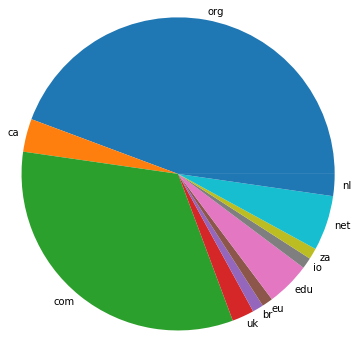
\includegraphics[width=7cm]{Figures/urls_1.png}
\end{figure}

\textbf{Code: tlds (pro-GM)}

\begin{lstlisting}
pro_urls = open("...\urls_pro_gmo.txt", "r", encoding="UTF-8")
pro_urls_lines = pro_urls.readlines()
tld_counts_pro = []
for url in pro_urls_lines:
    ind = [m.start() for m in re.finditer('/', url)][2]
    if url[ind-4] == ".":
        tld_counts_pro.append(url[ind-3:ind])
    if url[ind-3] == ".":
        tld_counts_pro.append(url[ind-2:ind])
print("total urls: " + str(len(pro_urls_lines))+"\n" )
print("Random sample of pro_gm urls:")
from random import sample
chosen_pro = sample(pro_urls_lines, 3)
for url in chosen_pro:
    print(url[0:-1])
counts_pro = Counter(tld_counts_pro)
print(counts_pro.most_common())
import matplotlib.pyplot as pyplot
plot2 = plt.pie([float(v) for v in counts_pro.values()],... 
labels=[k for k in counts_pro], labeldistance=1.05, radius=1.8)
\end{lstlisting}

\textbf{Output: tlds (pro-GM)}
\begin{footnotesize}
total urls: 91

Random sample of pro-gm urls:

https://bizfluent.com/info-8082116-positives-gmo.html\newline
https://www.marketplace.org/2016/08/09/world/sugar-beet-farmers-mull-objections-gmos\newline
https://www.bayer.com/en/position-on-genetic-engineering-straightforward.aspx
\end{footnotesize}

Top Level Domains (Pro-GM)\newline
----------------------------\newline
[('com', 50), ('org', 25), ('edu', 5), ('ca', 3), ('uk', 2), ('gov', 1), ('net', 1), ('cl', 1), ('in', 1), ('au', 1), ('ie', 1)]

\begin{figure}[H]
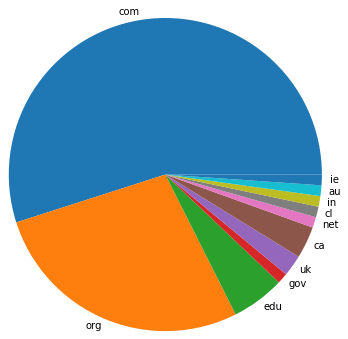
\includegraphics[width=7cm]{Figures/urls_2.png}
\end{figure}

\section{Keywords and top N-grams}

Top n-grams (sequences of \textit{n} words) were determined by taking the top frequencies on an absolute basis (i.e., not using a reference corpus for comparison). After removing stop words, the 20 most frequent uni-grams, bi-grams, and tri-grams (1-, 2-, and 3-word sequences) are determined for each corpus.

Code in this section is adapted from:\newline 
\small{https://medium.com/analytics-vidhya/
automated-keyword-extraction-from-articles-using-nlp-bfd864f41b34}

\textbf{Code: Keywords (anti-GM)}

\begin{lstlisting}

from sklearn.feature_extraction.text import CountVectorizer
import re
cv=CountVectorizer(max_df=0.8,stop_words=stop_words,
max_features=10000, ngram_range=(1,3))
X=cv.fit_transform(corpus_anti)
list(cv.vocabulary_.keys())[:10]
import pandas
#Most frequently occuring words
def get_top_n_words(corpus, n=None):
    vec = CountVectorizer().fit(corpus)
    bag_of_words = vec.transform(corpus)
    sum_words = bag_of_words.sum(axis=0) 
    words_freq = [(word, sum_words[0, idx]) for word, idx in      
                   vec.vocabulary_.items()]
    words_freq =sorted(words_freq, key = lambda x: x[1], 
                       reverse=True)
    return words_freq[:n]
#Convert most freq words to dataframe for plotting bar plot
top_words = get_top_n_words(corpus_anti, n=20)
top_df = pandas.DataFrame(top_words)
top_df.columns=["Word", "Freq"]
print(top_df)
#Barplot of most freq words
import seaborn as sns
sns.set(rc={'figure.figsize':(13,8)})
g = sns.barplot(x="Word", y="Freq", data=top_df)
g.set_xticklabels(g.get_xticklabels(), rotation=30)
\end{lstlisting}

\textbf{Output: Keywords (anti-GM)}

\begin{table}[H]
\begin{footnotesize}
\begin{tabular}{lll}
0  & seed        & 1749 \\
1  & food        & 1678 \\
2  & crop        & 1316 \\
3  & gm          & 1205 \\
4  & indigenous  & 1142 \\
5  & farmer      & 1107 \\
6  & people      & 1001 \\
7  & monsanto    & 656  \\
8  & right       & 630  \\
9  & traditional & 608  \\
10 & plant       & 540  \\
11 & use         & 510  \\
12 & also        & 499  \\
13 & land        & 483  \\
14 & genetically & 468  \\
15 & maize       & 465  \\
16 & cultural    & 454  \\
17 & company     & 424  \\
18 & community   & 416  \\
19 & corn        & 416 
\end{tabular}
\end{footnotesize}
\end{table}

\begin{figure}[H]
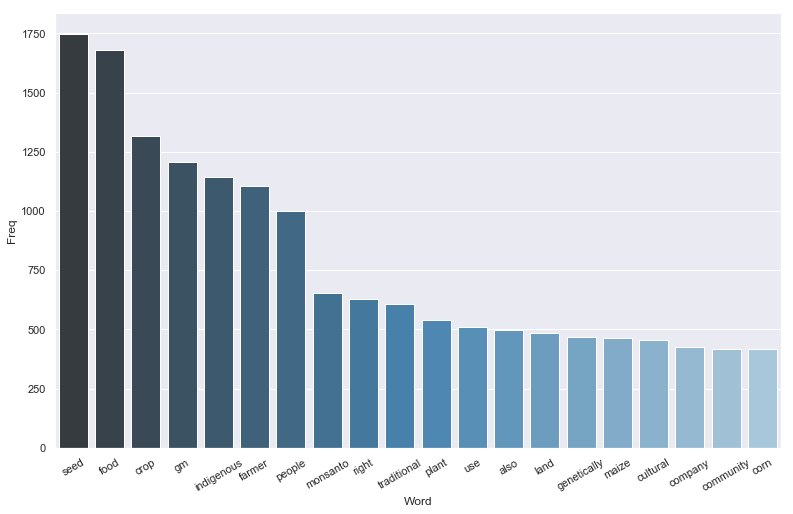
\includegraphics[width=14cm]{Figures/bar1.png}
\end{figure}

\textbf{Code: Keywords (pro-GM)}

\begin{lstlisting}
X=cv.fit_transform(corpus_pro)
list(cv.vocabulary_.keys())[:10]
#Convert most freq words to dataframe for plotting bar plot
top_wordsPRO = get_top_n_words(corpus_pro, n=20)
top_dfPRO = pandas.DataFrame(top_wordsPRO)
top_dfPRO.columns=["Word", "Freq"]
print(top_dfPRO)
#Barplot of most freq words
sns.set(rc={'figure.figsize':(13,8)})
g1 = sns.barplot(x="Word", y="Freq", data=top_dfPRO,  palette="Blues_d")
g1.set_xticklabels(g1.get_xticklabels(), rotation=30)
\end{lstlisting}

\textbf{Output: Keywords (pro-GM)}

\begin{table}[H]
\begin{footnotesize}
\begin{tabular}{lll}
0  & crop       & 1979 \\
1  & gm         & 1977 \\
2  & ha         & 1120 \\
3  & impact     & 991  \\
4  & technology & 712  \\
5  & million    & 708  \\
6  & use        & 688  \\
7  & food       & 685  \\
8  & ht         & 666  \\
9  & farmer     & 639  \\
10 & soybean    & 627  \\
11 & herbicide  & 618  \\
12 & year       & 617  \\
13 & cotton     & 566  \\
14 & cost       & 507  \\
15 & farm       & 498  \\
16 & carbon     & 498  \\
17 & yield      & 486  \\
18 & seed       & 469  \\
19 & country    & 456 
\end{tabular}
\end{footnotesize}
\end{table}

\begin{figure}[H]
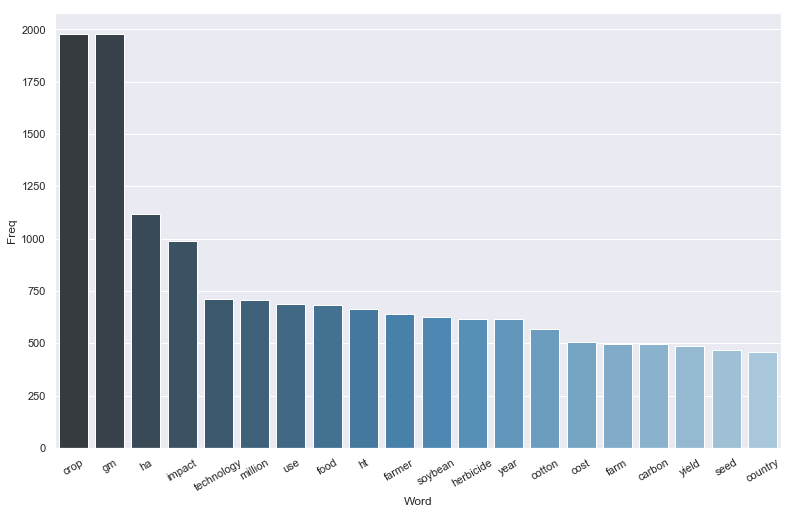
\includegraphics[width=14cm]{Figures/bar2.png}
\end{figure}

\textbf{Code: Bi-grams (anti-GM)}

\begin{lstlisting}
#Most frequently occurring Bi-grams
def get_top_n2_words(corpus, n=None):
    vec1 = CountVectorizer(ngram_range=(2,2),  
            max_features=2000).fit(corpus)
    bag_of_words = vec1.transform(corpus)
    sum_words = bag_of_words.sum(axis=0) 
    words_freq = [(word, sum_words[0, idx]) for word, idx in     
                  vec1.vocabulary_.items()]
    words_freq =sorted(words_freq, key = lambda x: x[1], 
                reverse=True)
    return words_freq[:n]
top2_words = get_top_n2_words(corpus_anti, n=20)
top2_df = pandas.DataFrame(top2_words)
top2_df.columns=["Bi-gram", "Freq"]
print(top2_df)
#Barplot of most freq Bi-grams
import seaborn as sns
sns.set(rc={'figure.figsize':(13,8)})
h=sns.barplot(x="Bi-gram", y="Freq", data=top2_df, palette="Blues_d")
h.set_xticklabels(h.get_xticklabels(), rotation=45)
\end{lstlisting}

\textbf{Output: Bi-grams (anti-GM)}

\begin{table}[H]
\begin{footnotesize}
\begin{tabular}{lll}
0  & indigenous people      & 576 \\
1  & gm crop                & 389 \\
2  & genetically modified   & 298 \\
3  & food sovereignty       & 164 \\
4  & per cent               & 159 \\
5  & non gm                 & 147 \\
6  & traditional food       & 141 \\
7  & genetically engineered & 129 \\
8  & indicator area         & 114 \\
9  & http www               & 112 \\
10 & food security          & 111 \\
11 & biocultural diversity  & 104 \\
12 & united state           & 92  \\
13 & right food             & 80  \\
14 & food system            & 79  \\
15 & traditional knowledge  & 77  \\
16 & indigenous community   & 72  \\
17 & et al                  & 72  \\
18 & non gmo                & 70  \\
19 & food production        & 67 
\end{tabular}
\end{footnotesize}
\end{table}

\begin{figure}[H]
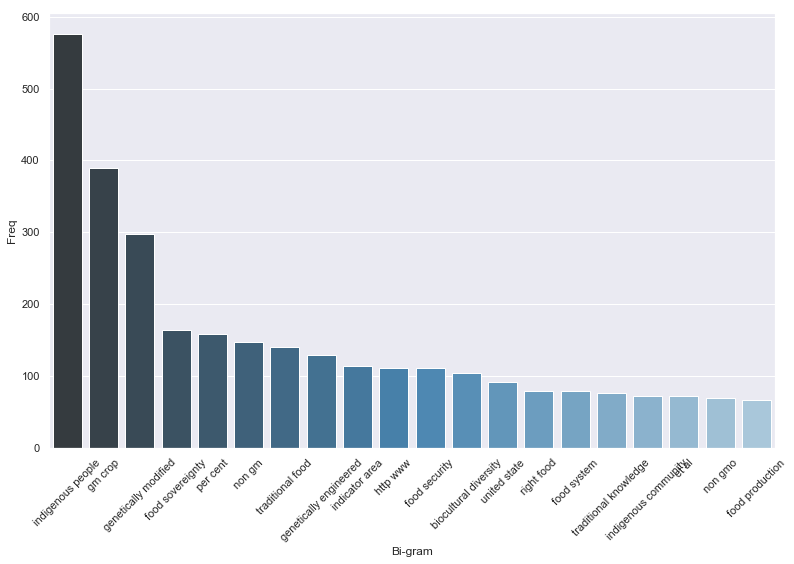
\includegraphics[width=14cm]{Figures/bar3.png}
\end{figure}

\textbf{Code: Bi-grams (pro-GM)}

\begin{lstlisting}
#Most frequently occurring Bi-grams
top2_wordsPRO = get_top_n2_words(corpus_pro, n=20)
top2_dfPRO = pandas.DataFrame(top2_wordsPRO)
top2_dfPRO.columns=["Bi-gram", "Freq"]
print(top2_dfPRO)
#Barplot of most freq Bi-grams
import seaborn as sns
sns.set(rc={'figure.figsize':(13,8)})
h=sns.barplot(x="Bi-gram", y="Freq", data=top2_dfPRO, palette="Blues_d")
h.set_xticklabels(h.get_xticklabels(), rotation=45)
\end{lstlisting}

\textbf{Output: Bi-grams (pro-GM)}

\begin{table}[H]
\begin{footnotesize}
\begin{tabular}{lll}
0  & gm ht                  & 569 \\
1  & gm crop                & 512 \\
2  & gm ir                  & 277 \\
3  & et al                  & 252 \\
4  & farm income            & 241 \\
5  & pg economics           & 209 \\
6  & crop impact            & 200 \\
7  & economics ltd          & 199 \\
8  & genetically modified   & 182 \\
9  & field eiq              & 175 \\
10 & ha ha                  & 162 \\
11 & ht soybean             & 158 \\
12 & biotech crop           & 138 \\
13 & million kg             & 136 \\
14 & environmental impact   & 134 \\
15 & active ingredient      & 129 \\
16 & cost saving            & 124 \\
17 & national academy       & 122 \\
18 & genetically engineered & 121 \\
19 & eiq ha                 & 120
\end{tabular}
\end{footnotesize}
\end{table}

\begin{figure}[H]
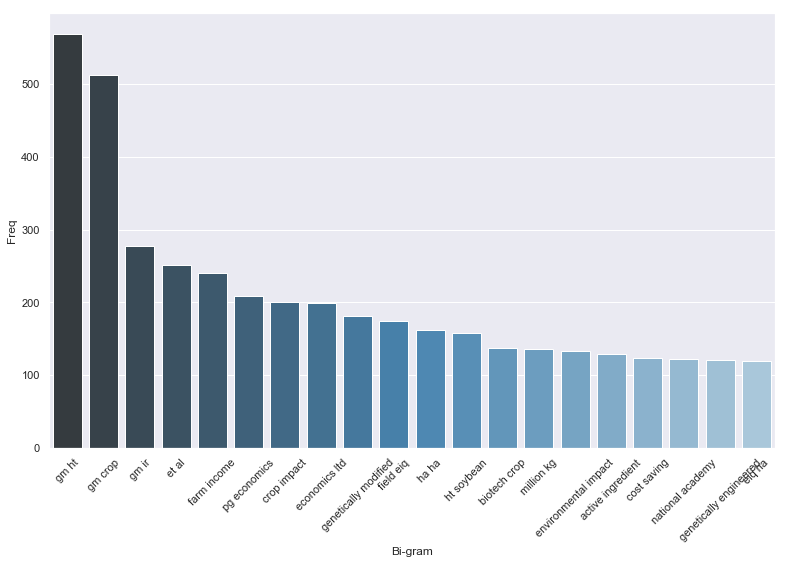
\includegraphics[width=14cm]{Figures/bar4.png}
\end{figure}

\textbf{Code: Tri-grams (anti-GM)}

\begin{lstlisting}
#Most frequently occurring Tri-grams
def get_top_n3_words(corpus, n=None):
    vec1 = CountVectorizer(ngram_range=(3,3), 
           max_features=2000).fit(corpus)
    bag_of_words = vec1.transform(corpus)
    sum_words = bag_of_words.sum(axis=0) 
    words_freq = [(word, sum_words[0, idx]) for word, idx in     
                  vec1.vocabulary_.items()]
    words_freq =sorted(words_freq, key = lambda x: x[1], 
                reverse=True)
    return words_freq[:n]
top3_words = get_top_n3_words(corpus_anti, n=20)
top3_df = pandas.DataFrame(top3_words)
top3_df.columns=["Tri-gram", "Freq"]
print(top3_df)
#Barplot of most freq Tri-grams
import seaborn as sns
sns.set(rc={'figure.figsize':(13,8)})
j=sns.barplot(x="Tri-gram", y="Freq", data=top3_df, palette="Blues_d")
j.set_xticklabels(j.get_xticklabels(), rotation=45)
\end{lstlisting}

\textbf{Output: Tri-grams (anti-GM)}

\begin{table}[H]
\begin{footnotesize}
\begin{tabular}{lll}
0  & genetically modified organism & 51 \\
1  & genetically modified seed     & 48 \\
2  & biocultural diversity toolkit & 44 \\
3  & genetically modified crop     & 42 \\
4  & genetically modified food     & 38 \\
5  & non gm crop                   & 37 \\
6  & agro ecological system        & 36 \\
7  & food agro ecological          & 34 \\
8  & growing gm crop               & 32 \\
9  & anti gm activism              & 31 \\
10 & indigenous people right       & 29 \\
11 & genetically engineered food   & 28 \\
12 & genetically engineered crop   & 28 \\
13 & food sovereignty critical     & 28 \\
14 & nd global consultation        & 27 \\
15 & intellectual property right   & 27 \\
16 & sovereignty critical dialogue & 27 \\
17 & gm activism mexico            & 26 \\
18 & right indigenous people       & 25 \\
19 & activism mexico colombia      & 25 \\
\end{tabular}
\end{footnotesize}
\end{table}

\begin{figure}[H]
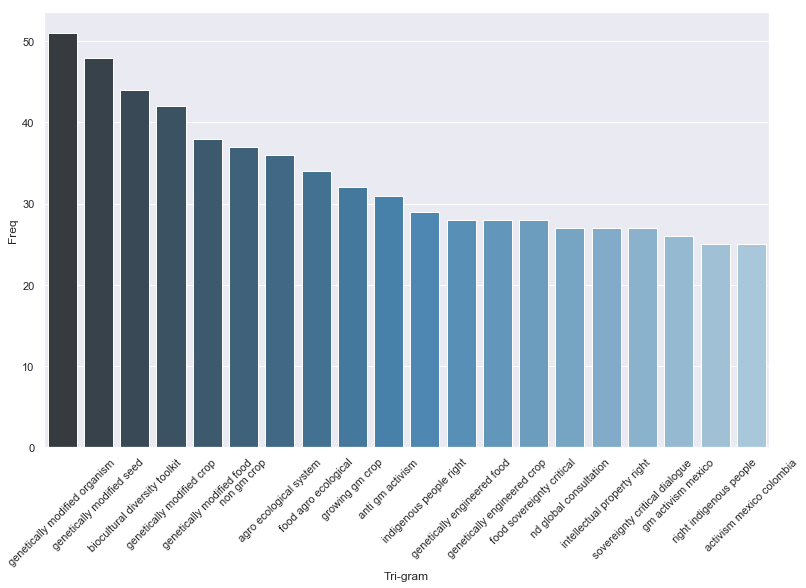
\includegraphics[width=14cm]{Figures/bar5.png}
\end{figure}

\textbf{Code: Tri-grams (pro-GM)}

\begin{lstlisting}
#Most frequently occurring Tri-grams
top3_wordsPRO = get_top_n3_words(corpus_pro, n=20)
top3_dfPRO = pandas.DataFrame(top3_wordsPRO)
top3_dfPRO.columns=["Tri-gram", "Freq"]
print(top3_dfPRO)
#Barplot of most freq Tri-grams
import seaborn as sns
sns.set(rc={'figure.figsize':(13,8)})
j=sns.barplot(x="Tri-gram", y="Freq", data=top3_dfPRO, palette="Blues_d")
j.set_xticklabels(j.get_xticklabels(), rotation=45)
\end{lstlisting}

\textbf{Output: Tri-grams (pro-GM)}

\begin{table}[H]
\begin{footnotesize}
\begin{tabular}{lll}
0  & pg economics ltd             & 199 \\
1  & gm crop impact               & 198 \\
2  & gm ht soybean                & 139 \\
3  & field eiq ha                 & 99 \\
4  & gm ir cotton                 & 95 \\
5  & genetically engineered crop  & 71 \\
6  & using gm ht                  & 71 \\
7  & impact using gm              & 69 \\
8  & farm income gain             & 65 \\
9  & national academy science     & 63 \\
10 & gm ir maize                  & 61 \\
11 & kg carbon ha                 & 61 \\
12 & farm income benefit          & 58 \\
13 & academy science engineering  & 54 \\
14 & science engineering medicine & 54 \\
15 & income impact using          & 53 \\
16 & carbon ha year               & 52 \\
17 & gm ht maize                  & 51 \\
18 & genetically modified crop    & 49 \\
19 & national academy press       & 49 \\
\end{tabular}
\end{footnotesize}
\end{table}


\begin{figure}[H]
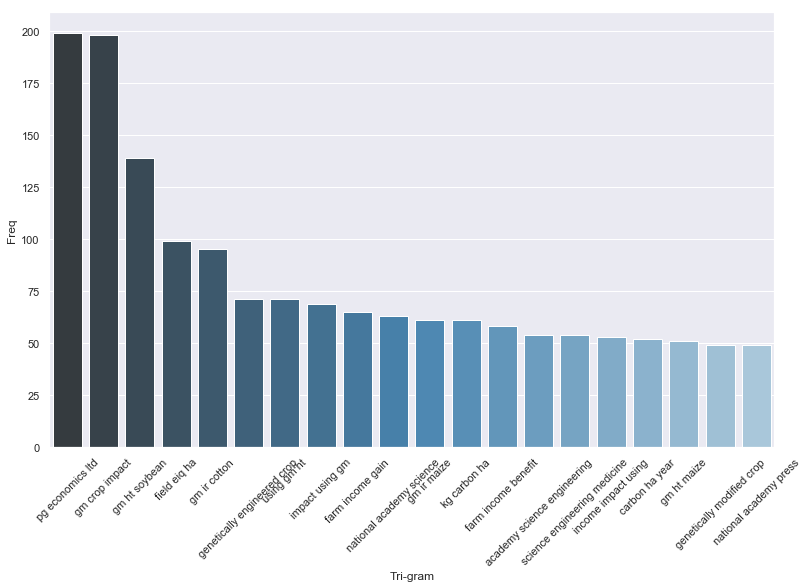
\includegraphics[width=14cm]{Figures/bar6.png}
\end{figure}

\section{Type-Token Ratio}
Lexical diversity is calculated through the type-token ratio (TTR). For this, the non-preprocessed texts were used so TTR values could be compared with other corpora/texts.

\textbf{Code: TTR}

\begin{lstlisting}
antiList = " ".join(anti_lines).split()
proList = " ".join(pro_lines).split()
# Yield successive n-sized 
# chunks from l. 
def divide_chunks(l, n): 
    # looping till length l 
        for i in range(0, len(l), n): 
            yield l[i:i + n] 
# n = how many elements in each list 
n = 2000
x = list(divide_chunks(antiList, n)) 
y = list(divide_chunks(proList, n)) 
TTRs = []
for chunk in x:
    wordsUnique = []
    for word in chunk:
        if word not in wordsUnique:
            wordsUnique.append(word)
    ttr=len(wordsUnique)/len(chunk)
    TTRs.append(ttr)
TTRsPro = []
for chunk in y:
    wordsUnique = []
    for word in chunk:
        if word not in wordsUnique:
            wordsUnique.append(word)
    ttr=len(wordsUnique)/len(chunk)
    TTRsPro.append(ttr)
antiLD = sum(TTRs) / len(TTRs)
proLD = sum(TTRsPro) / len(TTRsPro)
print("anti-GM Corpus: " + str(round(antiLD,2)))
print("pro-GM Corpus:  " + str(round(proLD,2)))
\end{lstlisting}

\textbf{Output: TTR for each subcorpus}

\begin{footnotesize}
anti-GM Corpus: 0.45\newline
pro-GM Corpus:  0.42
\end{footnotesize}

\section{Specialized Terminology}
A more direct measure of the presence of scientific terminology is comparison of the corpora with a dictionary of scientific terms. To conduct such a comparison, a molecular biology glossary is used which comprised of 170 terms. For each subcorpora, counts were taken for the frequency of glossary terms. 

To account for the different sizes of corpora, frequencies are based on a random sample of 100,000 tokens from each corpus. The average frequency was then calculated over 100 random samples.

For each corpus we output the counts (e.g., {gene:445}) to determine precisely which molecular biology terms appeared in each subcorpus. 

\textbf{Code: Specialized Terms}

\begin{lstlisting}
import random
from collections import Counter
f= open("...allTerms.txt", "r", encoding="UTF-8")
terms = f.readlines()
allTerms = [x.lower() for x in terms]
allTerms= [x.replace('\n', '') for x in allTerms]
print(str(len(terms)) + " terms in the dictionary\n") 
from random import sample
print("Random sample of terms:")
chose_terms = sample(terms, 3)
for i in chose_terms:
    print("-"+i[0:-1])
print("\n")
subList = []
counts_anti = []
counts_pro = []
words_anti = []
words_pro = []
size=100000
print("taking " + str(10)+ " samples of " +str(size) + " tokens..." + "\n")
def getCount(corpus, lst, words):
    for y in allTerms:
        if corpus.count(y) > 1:
            subList.append(y)
    samples = []
    i=0
    while i < 10:
        sampleRand=random.sample(corpus.split(), size)
        samples.append(sampleRand)
        i=i+1
    for sample in samples:
        count=0
        for z in subList:
            for q in sample:
                if z==q:
                    count=count+1
                    words.append(z)
        lst.append(count)
getCount(anti_textPre, counts_anti, words_anti)    
getCount(pro_textPre, counts_pro, words_pro)    
average = sum(counts_anti)/len(samples)
average_pro = sum(counts_pro)/len(samples)
print("average frequency (anti-GM): " +str(round(average,10)))
print("average frequency (pro-GM): " +str(round(average_pro,10)))
d1 = dict()
for i in words_anti:
  d1[i] = d1.get(i, 0) + 1
d2 = dict()
for i in words_pro:
  d2[i] = d2.get(i, 0) + 1
import operator
sorted_d1 = sorted(d1.items(), key=operator.itemgetter(1), reverse=True)
sorted_d2 = sorted(d2.items(), key=operator.itemgetter(1), reverse=True)
print("\n" + "Terms in the anti-GM corpus:")
print(sorted_d1)
print("\n" + "Terms in the pro-GM corpus:")
print(sorted_d2)
\end{lstlisting}

\textbf{Output: Specialized Terms (Molecular Biology)}
\begin{footnotesize}

170 terms in the dictionary

Random sample of terms:\newline
-Anneal\newline
-BAC\newline
-Acrylamide gels

taking 10 samples of 100000 tokens...

average frequency (anti-GM): 101.7\newline
average frequency (pro-GM): 439.0

Terms in the anti-GM corpus:
[('gene', 477), ('expression', 99), ('genome', 87), ('hybridization', 66), ('processing', 54), ('message', 35), ('insert', 34), ('restriction', 34), ('sequence', 25), ('marker', 23), ('library', 16), ('primer', 13), ('promoter', 13), ('translation', 13), ('cap', 9), ('nt', 8), ('plasmid', 6), ('genotype', 5)]

Terms in the pro-GM corpus:
[('nt', 2334), ('gene', 1234), ('genome', 228), ('sequence', 128), ('expression', 124), ('processing', 94), ('cap', 90), ('message', 46), ('insert', 40), ('marker', 32), ('lambda', 10), ('screening', 10), ('hybridization', 7), ('library', 7), ('promoter', 6)]
\end{footnotesize}

\textbf{Code: Concondance lines of \textit{NT}}

The output above suggests that the pro-GM corpus has over 4 times the number of terms. However, from the output counts we see that 'NT' (abbr. for nucleotide) is disproportionate in the pro-GM corpus. To investigate we look at the context of where 'NT' appears in the text.

Below we take a random sample of concordances of 'NT'. We see that is not used as an abbreviation for nucleotide; rather, it NT means frequently means no-till in this corpus. Moreover, we see that there are only 128 matches, far fewer than indicated in the counts above. This means that 'nt' (as a lowercase substring) was counted above where is had little to do with 'NT' meaning nucleotide.
\newline
\begin{lstlisting}
nt_concord = []
for i in range(0,len(proList)):
    if proList[i] == "NT":
        snippet = " ".join(proList[i-15:i+15])
        loc = snippet.index("NT")
        line = snippet[loc-25:loc+32]
        if line not in nt_concord:
            nt_concord.append(line)
print("count:" +str(len(nt_concord))+ "\n")
print('Random sample:' ) 
from random import sample
chosen_nt = sample(nt_concord, 10)
for i in chosen_nt:
    print(i)
\end{lstlisting}

\textbf{Output: Concondance lines of \textit{NT}}

\begin{footnotesize}
count:128

Random sample:

relating to the use of NT systems 111) and this identif\newline
\ \ ith the premise that NT results in positive carbon se\newline
.......... systems. The NT system stored and retained 7.\newline
\ area is in continuous NT crop rotation, the full SOC b\newline
estimated that RT or NT typically uses 19 to 38 litre\newline
been by farmers using NT systems (GM HT cultivars acco\newline
8) work also compared NT and full-inversion tillage (F\newline
Mathew et al. (2012)). NT soils are more biologically a\newline
014 Total Assumption: NT = +175 kg carbon/ha/yr, CT = \newline
rch comparing CT with NT has demonstrated that NT resu\newline
\end{footnotesize}

\textbf{Code: Terms (Molecular Biology) - Adjusted}

\begin{lstlisting}
allTerms.remove('nt')
subList = []
counts_anti = []
counts_pro = []
words_anti = []
words_pro = []
getCount(anti_textPre, counts_anti, words_anti)    
getCount(pro_textPre, counts_pro, words_pro)
average = sum(counts_anti)/len(samples)
average_pro = sum(counts_pro)/len(samples)
print("Results after removing 'NT' from the terms:\n")   
print("average frequency (anti-GM): " +str(round(average,10)))
print("average frequency (pro-GM): " +str(round(average_pro,10)))
\end{lstlisting}

\textbf{Output: Terms (Molecular Biology) - Adjusted}

\begin{footnotesize}
Results after removing 'NT' from the terms:

average frequency (anti-GM): 79.3\newline
average frequency (pro-GM): 205.6
\end{footnotesize}

\textbf{Code: Terms (Agrochemicals)}

The same dictionary process was repeated with a glossary of agrochemicals. Common names of 2,498 herbicides and pesticides were collected and frequencies obtained for both subcorpora.

\begin{lstlisting}
g= open("...herbPestNames.txt", "r", encoding="UTF-8")
termsHerb = g.readlines()
allTerms = [x.lower() for x in termsHerb]
allTerms= [x.replace('\n', '') for x in allTerms]
print(str(len(termsHerb)) + " terms in the dictionary\n") 
from random import sample
print("Random sample of terms:")
chose_termsHerb = sample(termsHerb, 3)
for i in chose_termsHerb:
    print("-"+i[0:-1])
print("\n")
subList = []
counts_anti = []
counts_pro = []
words_anti = []
words_pro = []
size=100000
print("taking " + str(10)+ " samples of " +str(size) + " tokens..." + "\n")
getCount(anti_textPre, counts_anti, words_anti)    
getCount(pro_textPre, counts_pro, words_pro)
average = sum(counts_anti)/len(samples)
average_pro = sum(counts_pro)/len(samples)
print("average frequency (anti-GM): " +str(round(average,10)))
print("average frequency (pro-GM): " +str(round(average_pro,10)))
d1 = dict()
for i in words_anti:
  d1[i] = d1.get(i, 0) + 1
d2 = dict()
for i in words_pro:
  d2[i] = d2.get(i, 0) + 1
import operator
sorted_d1 = sorted(d1.items(), key=operator.itemgetter(1), reverse=True)
sorted_d2 = sorted(d2.items(), key=operator.itemgetter(1), reverse=True)
print("\n" + "Terms in the anti-GM corpus:")
print(sorted_d1)
print("\n" + "Terms in the pro-GM corpus:")
print(sorted_d2)
\end{lstlisting}

\textbf{Output: Terms (Agrochemicals)}

\begin{footnotesize}

2498 terms in the dictionary

Random sample of terms:\newline
-proparthrin\newline
-cicloheximide\newline
-jasmolin II

taking 10 samples of 100000 tokens...

average frequency (anti-GM): 91.9\newline
average frequency (pro-GM): 595.6

Terms in the anti-GM corpus:\newline
[('glyphosate', 710), ('glufosinate', 102), ('dicamba', 32), ('paraquat', 22), ('atrazine', 22), ('ddt', 21), ('dep', 10)]

Terms in the pro-GM corpus:\newline
[('glyphosate', 3744), ('glufosinate', 660), ('atrazine', 232), ('clethodim', 138), ('fomesafen', 114), ('chlorimuron', 102), ('flumioxazin', 100), ('trifluralin', 96), ('acetochlor', 80), ('pendimethalin', 64), ('prometryn', 58), ('dicamba', 52), ('sulfentrazone', 50), ('metolachlor', 39), ('imazethapyr', 36), ('metsulfuron', 36), ('imidacloprid', 35), ('diuron', 32), ('cypermethrin', 31), ('methomyl', 30), ('acetamiprid', 26), ('chlorpyrifos', 26), ('acc', 26), ('diafenthiuron', 17), ('deltamethrin', 16), ('buprofezin', 14), ('acephate', 12), ('endosulfan', 12), ('phoxim', 12), ('abamectin', 12), ('metaflumizone', 11), ('parathion', 11), ('cyhalothrin', 10), ('monocrotophos', 9), ('chlorfenapyr', 7), ('cma', 6)]

\end{footnotesize}

\section{Concordances of \textit{ecological} \& \textit{biological}}
Concordances of the words \textit{ecological} and \textit{biological} can provide insight into how living systems are referred to linguistically. 

\textbf{Code: Concordances of \textit{ecological}}

\begin{lstlisting}
anti_low = anti_text.lower()
anti_list = anti_low.split()
culture_concord = []
for i in range(0,len(anti_list)):
    if anti_list[i] == "culture":
        snippet = " ".join(anti_list[i-15:i+15])
        loc = snippet.index("culture")
        line = snippet[loc-25:loc+32]
        if line not in culture_concord:
            culture_concord.append(line)
print('ANTI-GM Corpus' + "\n--------------" + "\n")             
print("Total unqiue lines: " + str(len(culture_concord)) + "\n")
print('Random sample:' + "\n") 
from random import sample
chosen_cult = sample(culture_concord, 10)
for i in chosen_cult:
    print(i)
pro_low = pro_text.lower()
pro_list = pro_low.split()
culture_concord_pro = []
for i in range(0,len(pro_list)):
    if pro_list[i] == "culture":
        snippet = " ".join(pro_list[i-15:i+15])
        loc = snippet.index("culture")
        line = snippet[loc-25:loc+32]
        if line not in culture_concord_pro:
            culture_concord_pro.append(line)
print('\nPRO-GM Corpus' + "\n--------------" + "\n")            
print("Total unqiue lines: " + str(len(culture_concord_pro)) + "\n")
for i in culture_concord_pro:
    print(i)
\end{lstlisting}

\textbf{Output: Concordances of \textit{ecological}}

\begin{footnotesize}
ANTI-GM Corpus\newline
-----------------------

Total unique lines: 107

Random sample:

g role culture food agro ecological system sound alert po\newline
tion meet need community ecological refugia pastoral netw\newline
ustomary law traditional ecological knowledge legal frame\newline
pacific northwest social ecological system ecology societ\newline
challenge coupled social ecological system address challe\newline
ge traditional food agro ecological system number differe\newline
ay france gmos demanding ecological approach agriculture \newline
shock like flood drought ecological farming model based b\newline
igenous people food agro ecological system indigenous peo\newline
on feeding volatile city ecological sustainability subsis\newline
ing haiti cannot sustain ecological destruction impositio\newline
m assessment traditional ecological knowledge zerner godo\newline
nsidered necessary sound ecological management riddell ec\newline
ell song dance myth agro ecological food system offer sig

PRO-GM Corpus\newline
-----------------------

Total unique lines: 14

edness combined volatile ecological climate socioeconomic\newline
tton htm shetty pk socio ecological implication pesticide\newline
 industrial biotech agro ecological paradigm drawing aspe\newline
 different crop one many ecological farming practice us k\newline
g people real food based ecological agriculture address m\newline
esting climate resilient ecological agriculture empowerin\newline
 sheet describing health ecological environmental effect \newline
onent consumer component ecological component component e\newline
age farm worker consumer ecological component eiq c dt dt\newline
e ability absorbed plant ecological component model compo\newline
ion farm worker consumer ecological average eiq value pre\newline
et al assessing economic ecological impact herbicide tole\newline
hed march concluded agro ecological farming system feed w
\end{footnotesize}

\textbf{Code: Concordances of \textit{biological}}

\begin{lstlisting}
getConcord("biological", bio_concord, bio_concord_pro)
print('ANTI-GM Corpus' + "\n--------------" + "\n")             
print("Total unique lines: " + str(len(bio_concord)) + "\n")
print('Random sample:' + "\n") 
from random import sample
chosen_bio = sample(bio_concord, 10)
for i in chosen_bio:
    print(i)
pro_low = pro_text.lower()
pro_list = pro_low.split()
print('\nPRO-GM Corpus' + "\n--------------" + "\n")            
print("Total unique lines: " + str(len(bio_concord_pro)) + "\n")
for i in bio_concord_pro:
    print(i)
\end{lstlisting}

\textbf{Output: Concordances of \textit{biological}}

\begin{footnotesize}

ANTI-GM Corpus\newline
-----------------------

Total unique lines: 94

Random sample:

rge share world cultural biological diversity yet largely\newline
y human culture language biological cultural linguistic b\newline
tal knowledge convention biological diversity hlclep firs\newline
or due instance chemical biological function kill growing\newline
ranking position country biological language diversity co\newline
ndigenous culture people biological productive resource s\newline
ervation sustainable use biological diversity promote wid\newline
used organic farmer form biological pest control crop gen\newline
ference party convention biological diversity prepared dr\newline
mmunication need however biological specie human language

PRO-GM Corpus\newline
-----------------------

Total unique lines: 10

sustainable modification biological resource going much p\newline
 really dad arguing need biological solution like gm redu\newline
truction expand research biological science based program\newline
enta innovative chemical biological solution aligning new\newline
peed automated synthesis biological method prepare quanti\newline
 change plant metabolism biological activity complex regi\newline
anic farmer e g new type biological control tested decade\newline
 country use alternative biological cultural control meas\newline
examination data diverse biological societal aspect curre\newline
arch study found adverse biological social effect ge crop
\end{footnotesize}

\textbf{Code: Concordances of \textit{culture}}

\begin{lstlisting}
culture_concord = []
culture_concord_pro = []
getConcord("culture", culture_concord, culture_concord_pro)
print('ANTI-GM Corpus' + "\n--------------" + "\n")             
print("Total unique lines: " + str(len(culture_concord)) + "\n")
print('Random sample:' + "\n") 
from random import sample
chosen_culture = sample(culture_concord, 10)
for i in chosen_culture:
    print(i)
pro_low = pro_text.lower()
pro_list = pro_low.split()
print('\nPRO-GM Corpus' + "\n--------------" + "\n")            
print("Total unique lines: " + str(len(culture_concord_pro)) + "\n")
for i in culture_concord_pro:
    print(i)
\end{lstlisting}

\textbf{Output: Concordances of \textit{culture}}

\begin{footnotesize}

ANTI-GM Corpus\newline
-----------------------

Total unique lines: 211

Random sample:

ation science technology culture including seed medicine\newline 
nt emphasizes importance culture needed value identified\newline
 world difference nature culture benefit human life yet m\newline
 people without language culture cannot survive assembly\newline 
edge connection language culture environment local level\newline 
 corn core rural mexican culture millennium every ground\newline 
able training accordance culture order achieve technical\newline 
g deemed legal done harm culture community gmos different\newline
t recognition importance culture development un education\newline
 acceptable within given culture accessibility food way s

PRO-GM Corpus\newline
-----------------------

Total unique lines: 4

gy seed teach farmer new culture practice get completely\newline
op tool including tissue culture diagnostics genomics mol\newline
formed cell grown tissue culture become plantlet eventual\newline
icroorganism e g starter culture changed precisely random
\end{footnotesize}


\textbf{Code: Concordances of \textit{culture}}

\begin{lstlisting}
indig_concord = []
indig_concord_pro = []
getConcord("indigenous", indig_concord, indig_concord_pro)
print('ANTI-GM Corpus' + "\n--------------" + "\n")                     
print("Total unique lines: " + str(len(indig_concord)) + "\n")
print('Random sample:' + "\n") 
from random import sample
chosen_indig = sample(indig_concord, 10)
for i in chosen_indig:
    print(i)
pro_low = pro_text.lower()
pro_list = pro_low.split()
print('\nPRO-GM Corpus' + "\n--------------" + "\n")            
print("Total unique lines: " + str(len(indig_concord_pro)) + "\n")
for i in indig_concord_pro:
    print(i)
\end{lstlisting}

\textbf{Output: Concordances of \textit{indigenous}}

\begin{footnotesize}

ANTI-GM Corpus\newline
-----------------------

Total unique lines: 784

Random sample:

deral level exist mexico indigenous population living wit\newline
support system mean many indigenous migrant live distress\newline
uld undermine livelihood indigenous people genetic use re\newline
y program restrict limit indigenous people use access lan\newline
n implemented adequately indigenous people adopted vote f\newline
meet cultural aspiration indigenous people livestock rais\newline
g common property regime indigenous local community terri\newline
subsistence food carried indigenous people percentage tra\newline
ce however effect factor indigenous people role indigenou\newline
ecognized un declaration indigenous people rarely consult

PRO-GM Corpus\newline
-----------------------

Total unique lines: 0

\end{footnotesize}


\section{Distribution of Geographic Entities}
Some quantitative analysis provides a better view concentration and distribution of countries in the corpus. Using the Python software package \textit{geotext} country and city names are extracted from each subcorpus. City names are counted only if the population is greater than 500,000. The cities are then referenced back to their countries and the resulting countries are counted and sorted for each subcorpus.

\textbf{Code: Countries in the Corpus}

\begin{lstlisting}
# import libraries for entity recognition and country codes
import sys
from geotext import GeoText
from iso3166 import countries
from tabulate import tabulate
# read corpus and data
anti_file = "...\anti_gmo.txt"
pro_file = "...\pro_gmo.txt"
cities_file = "...worldcities.csv"
# create lists as global 
freqMaster = {}
freq_anti = {} 
freq_pro = {} 
freqCities_anti = {}
freqCities_pro = {}
countByCit_anti = []
countByCit_pro = []
# define function
def geo(corpusFile, targList, wc, freq, freqCities):
    with open (corpusFile, "r", encoding="utf8") as f:
        lines = f.readlines()
        text=" ".join(lines)
        wordCount = len(text.split())/1000
        wc.append(wordCount)
        # get reference list of all country names (iso3166)
        refList = []
        for c in countries:
            refList.append(c[-1])
        # get countries and cities from corpus 
        places = GeoText(text)
        countriesAll = places.countries
        citiesAll = places.cities
        # import cities to cross-reference
        import pandas
        colnames = ["city","city_ascii","lat","lng","country","iso2","iso3",
        "admin_name","capital","population","id"]
        data = pandas.read_csv(cities_file, names=colnames)
        names = data.city.tolist()
        country = data.country.tolist()
        population = data.population.tolist()
        countriesByCities = []
        for city in citiesAll:
            if city in names:
                ind=names.index(city)
                if float(population[ind]) > 500000:
                    #print(names[ind] + "," + " " + country[ind] +"," + " " +
                    str(population[ind]))
                    countriesByCities.append(country[ind])
        # custom replace country names of with iso3166
        countriesAll = ["Bolivia, Plurinational State of" if x=="Bolivia" 
        else x for x in countriesAll]
        countriesAll = ["United States of America" if x=="United States" 
        else x for x in countriesAll]
        countriesByCities = ["United States of America" if x=="United States" 
        else x for x in countriesByCities]
        countriesAll = ["Tanzania, United Republic of" if x=="Tanzania" 
        else x for x in countriesAll]
        countriesAll = ["Venezuela, Bolivarian Republic of" if x=="Venezuela" 
        else x for x in countriesAll]
        countriesByCities = ["Venezuela, Bolivarian Republic of" if x=="Venezuela"
         else x for x in countriesByCities]
        countriesAll = ["Viet Nam" if x=="Vietnam" else x for x in countriesAll]
        countriesAll = ["Syrian Arab Republic" if x=="Syria" 
        else x for x in countriesAll]
        countriesAll = ["United Kingdom of Great Britain and Northern Ireland" 
        if x=="United Kingdom" else x for x in countriesAll]
        countriesByCities = ["United Kingdom of Great Britain and Northern Ireland"
        if x=="United Kingdom" else x for x in countriesByCities]
        countriesAll = ["Korea, Republic of" if x=="South Korea" 
        else x for x in countriesAll]
        countriesAll = ["Czechia" if x=="Czech Republic" else x for x in countriesAll]
        countriesAll = ["Russian Federation" if x=="Russia" else x for x in countriesAll]
        countriesAll = ["Micronesia, Federated States of" if x=="Micronesia" 
        else x for x in countriesAll]
        if "Vatican" in countriesAll:
            countriesAll.remove("Vatican")
        # find country names in the corpus that do not correspond to an iso3166 name
        # print any suggestions for custom name replace
        noFits = []
        for x in countriesAll:
            if x not in refList:
                if x not in noFits:
                    noFits.append(x)
        if len(noFits)>0:
            print("No country code found for: ")
            for x in noFits:
                print(x)
        for x in noFits:
            for y in refList:
                if x in y:
                    print("try: " + y)
        # create dict with country counts {"CAN":23, USA:89, ...} 
        # dict for both country mentions and city mentions
        for c in countriesAll: 
            item = countries.get(c)[2]
            if (item in freq): 
                freq[item] += 1
            else: 
                freq[item] = 1
            if (item in freqMaster): 
                freqMaster[item] += 1
            else: 
                freqMaster[item] = 1
        for c in countriesByCities: 
            item = countries.get(c)[2]
            if (item in freqCities): 
                freqCities[item] += 1
            else: 
                freqCities[item] = 1
            if (item in freqMaster): 
                freqMaster[item] += 1
            else: 
                freqMaster[item] = 1
        tab = []
        sorted_freqMaster = sorted(freqMaster.items(), 
        key=operator.itemgetter(1), reverse=True)
        for key, value in sorted_freqMaster[0:10]:
            tab.append([countries.get(key)[0], round(value/wc[0],2)]])
        print(tabulate(tab, headers=['Country', 'Freq.']))
        for i in countriesByCities:
            targList.append(i)
print('ANTI-GM Corpus' + "\n")   
geo(anti_file, countByCit_anti, wc_anti, freq_anti, freqCities_anti)
print("\n"+'PRO-GM Corpus' + "\n")   
geo(pro_file, countByCit_pro, wc_pro, freq_pro, freqCities_pro)
\end{lstlisting}

\textbf{Output: Countries in the Corpus}

\begin{footnotesize}
ANTI-GM Corpus\newline
-----------------------

\begin{table}[H]
\begin{footnotesize}
\begin{tabular}{ll}

\textbf{Country}         & \textbf{Freq.} \\
Mexico                   & 0.82            \\
United States of America & 0.70           \\
Canada                   & 0.45           \\
India                    & 0.39           \\
Colombia                 & 0.30           \\
Nepal                    & 0.28           \\
Argentina                & 0.27           \\
Haiti                    & 0.25           \\
Brazil                   & 0.20           \\
Guatemala                & 0.17

\end{tabular}
\end{footnotesize}
\end{table}

PRO-GM Corpus\newline
-----------------------

\begin{table}[H]
\begin{footnotesize}
\begin{tabular}{ll}

\textbf{Country}         & \textbf{Freq.} \\
Argentina                & 1.04            \\
Canada                   & 0.91           \\
United States of America & 0.77            \\
Brazil                   & 0.67            \\
India                    & 0.60           \\
Australia                & 0.39           \\
South Africa             & 0.38           \\
Mexico                   & 0.34           \\
China                    & 0.32            \\
Philippines              & 0.29

\end{tabular}
\end{footnotesize}
\end{table}

\end{footnotesize}


\textbf{Code: North/South Geographic Split}

\begin{lstlisting}
import country_converter as cc
def nsSplit(freq, wc, freqCities, countByCit):
    cont = cc.convert(names = countByCit, to = 'UNregion')
    globNorth = 0
    globSouth = 0
    for c in cont:
        if c=="Northern America" or "Europe" in c:
            globNorth=globNorth+1
        else:
            globSouth=globSouth+1
    tab = []
    tab.append([round(100*globNorth/len(cont),2), round(100*globSouth/len(cont),2)])
    print(tabulate(tab, headers=['North (%)', 'South (%)']))
    ## get variation coefficient ##
    import statistics 
    # calculating deviation and variance
    sample = [] 
    countryFreqs = freq.values()
    for i in countryFreqs:
        sample.append(i/wc[0])
    mean = sum(sample)/len(sample)
    stdev = statistics.stdev(sample)
    coeff =stdev/mean
    # Prints standard deviation 
    # xbar is set to default value of 1 
    stddev = statistics.stdev(sample)
    print("\n"+"For the countries: ")
    print("Standard Deviation is % s " % (round(stddev,2))) 
    print("The coefficient of variation (CV) is " +  str(round(coeff,2)) +  "\n") 
    sample2 = [] 
    cityFreqs = freqCities.values()
    for i in cityFreqs:
        sample2.append(i/wc[0])
    mean2 = sum(sample2)/len(sample2)
    stdev2 = statistics.stdev(sample2)
    coeff2=stdev2/mean2
print('ANTI-GM Corpus' + "\n")       
nsSplit(freq_anti, wc_anti, freqCities_anti, countByCit_anti)
print('\nPRO-GM Corpus' + "\n")       
nsSplit(freq_pro, wc_pro, freqCities_pro, countByCit_pro)
\end{lstlisting}

\textbf{Output: North/South Geographic Split}

\begin{footnotesize}

ANTI-GM Corpus

\begin{table}[h]
\begin{footnotesize}
\begin{tabular}{ll}
\textbf{North (\%)} & \textbf{South (\%)} \\
61.99              & 38.01             
\end{tabular}
\end{footnotesize}
\end{table}

Standard Deviation is 0.12 \newline
The coefficient of variation (CV) is 1.87

PRO-GM Corpus

\begin{table}[h]
\begin{footnotesize}
\begin{tabular}{ll}
\textbf{North (\%)} & \textbf{South (\%)} \\
87.39            & 12.61             
\end{tabular}
\end{footnotesize}
\end{table}

Standard Deviation is 0.21 \newline
The coefficient of variation (CV) is 1.75

\end{footnotesize}

\textbf{Code: Shannon's Diversity Index}

\begin{lstlisting}
## calculating diversity of data
def divers(freqCities, wc):
    countryFreqs = []
    for i in freqCities.values():
        countryFreqs.append(i/wc)
    sumFreqs=sum(countryFreqs)
    n=len(countryFreqs)
    #average=sum(countryFreqs)/len(countryFreqs)
    proportions=[]
    for i in countryFreqs:
        proportions.append(i/sumFreqs)
    #print(proportions)
    import math
    listofzeros = [0] * (195-len(proportions))
    calcs = []
    for p in proportions:
        calc = p*(math.log(p))
        calcs.append(calc)
    final=listofzeros+calcs
    H1=-1*sum(final)
    print(round(H1,2))
    E=H1/math.log(195)
    print(round(E,2))
print('ANTI-GM Corpus') 
divers(freqCities_anti,wc_anti[0]*1000)
print('\nPRO-GM Corpus') 
divers(freqCities_pro,wc_pro[0]*1000
\end{lstlisting}

\textbf{Output:  Shannon's Diversity Index}
\begin{footnotesize}


ANTI-GM Corpus\newline
2.61\newline
0.49

PRO-GM Corpus\newline
1.3\newline
0.25

\end{footnotesize}


\section{Temporal Horizons \& Historical Context}

\textbf{Code: Concordances of \textit{centur*}}

\begin{lstlisting}
anti_file = "...\anti_gmo.txt"
pro_file = ...\pro_gmo.txt"
centur_concord = []
centur_concord_pro = []
def getConcordWildcard(file, targTerm, c1):
    with open (file, "r", encoding="utf8") as f:
        lines = f.readlines()
        text=" ".join(lines)
        low = text.lower()
        listsp = low.split()
        for i in range(0,len(listsp)):
            if targTerm in listsp[i]:
                snippet = " ".join(listsp[i-15:i+15])
                loc = snippet.index(targTerm)
                line = snippet[loc-25:loc+32]
                if line not in c1:
                    c1.append(line)
getConcordWildcard(anti_file, 'centur', centur_concord)
print('ANTI-GM Corpus' + "\n--------------" + "\n")                     
print("Total unique lines: " + str(len(centur_concord)) + "\n")
for i in centur_concord:
    print(i)
getConcordWildcard(pro_file, 'centur', centur_concord_pro)
print('\nANTI-GM Corpus' + "\n--------------" + "\n")                     
print("Total unique lines: " + str(len(centur_concord_pro)) + "\n")
for i in centur_concord_pro:
    print(i)
\end{lstlisting}

\textbf{Output: Concordances of \textit{centur*}}
\begin{footnotesize}
ANTI-GM Corpus\newline
-----------------------

Total unique lines: 34

e been enriched over the centuries through the abundant b\newline
ict (spanish in the 16th century, expropriation of land i\newline
economies since the 16th century, they have retained exte\newline
hich are the products of centuries of deliberate breeding\newline
eations that encapsulate centuries of historical events a\newline
odels at the turn of the century: individual property mod\newline
nt in panama in the 21st century. bioscience 51: 389-398.\newline
e first half of the 20th century, seeds were overwhelming\newline
llion by the turn of the century and that almost 1 billio\newline
eceived in the last half century. sustainable agriculture\newline
 that have been used for centuries. no-till farming is pr\newline
lture over the course of centuries, europeans have found \newline
nineteenth and twentieth centuries in europe, the man-mad\newline
in it. in mid-nineteenth century america, the natural won\newline
. in the late nineteenth century, the preservation of unt\newline
nforced in the twentieth century through the ways that ea\newline
tices sustain. twentieth-century philosophy in central eu\newline
 motifs of the twentieth century — that technology by its\newline
st half of the twentieth century to exercise precaution a\newline
y had depended on it for centuries. therefore it was very\newline
rsity over the twentieth century. now,just nine crops com\newline
to local conditions over centuries). these were rejected \newline
eds from their crops for centuries is at stake (as gmo cr\newline
ans beginning in the 8th century. 3. the ideological pare\newline
s, “during the past five centuries, while our people have\newline
r the course of the 20th century, according to the fao, a\newline
r they are the result of centuries of traditional plant b\newline
oped throughout the 20th century owe their origin to publ\newline
users guide for the 21st century31 argue, such a mindset \newline
ser’s guide for the 21st century. harry n. abrams, inc. 3\newline
he beginning of the 20th century, the world has lost 90\%\newline
rsity over the twentieth century. now, just nine crops co\newline
ich emerged in sixteenth century europe. i prefer the com\newline
l mexico. in the late 19 century into the contemporary pe

PRO-GM Corpus\newline
-----------------------

Total unique lines: 9

erspectives for the 21st century. session 17. 497-499. qa\newline
obal) by the end of this century in 2100 – global food se\newline
techniques in eighteenth century britain that brought abo\newline
ited states reflect many centuries of plant modification \newline
70 and 100 percent by midcentury. in particular, the rapi\newline
ple by the middle of the century. in one of his most ambi\newline
n the middle of the 20th century are the main reason that\newline
at have been planted for centuries. doohan looks at them \newline
 human foods in the 21st century: a review. biotechnol. a
\end{footnotesize}

\textbf{Code: Years in the Corpus}

\begin{lstlisting}
from operator import itemgetter
from collections import defaultdict
yearsf = "...\xseries.csv"
def plot_timeline(dataset, **kwargs):
    outpath = kwargs.pop('savefig', None)  # Save the figure as an SVG
    colors  = kwargs.pop('colors', {})     # Plot the colors for the series.
    series  = set([])                      # Figure out the unique series
    # Bring the data into memory and sort
    dataset = sorted(list(dataset), key=itemgetter(0))
    # Make a first pass over the data to determine number of series, etc.
    for _, source, category in dataset:
        series.add(source)
        if category not in colors:
            colors[category] = 'k'
    # Sort and index the series
    series  = sorted(list(series))
    # Create the visualization
    x = []  # Scatterplot X values
    y = []  # Scatterplot Y Values
    c = []  # Scatterplot color values
    # Loop over the data a second time
    for timestamp, source, category in dataset:
        x.append(timestamp)
        y.append(series.index(source))
        c.append(colors[category])
    plt.figure(figsize=(16,6))
    plt.title(kwargs.get('title', "Years in the Corpus"))
    plt.ylim((-1,len(series)))
    plt.xlim((1800, dataset[-1][0]+10))
    plt.yticks(range(len(series)), series)
    plt.scatter(x, y, color=c, alpha=0.85, s=10)
    if outpath:
        return plt.savefig(outpath, format='svg', dpi=1600)
    return plt
if __name__ == '__main__':
    colors = {'red': 'r', 'blue': 'b', 'green': 'g'}
    with open(yearsf, 'r') as f:
        reader = csv.reader(f)
        plt = plot_timeline([
            (float(row[0]), row[1], row[2])
            for row in reader
        ], colors=colors)
        plt.show()
\end{lstlisting}

\textbf{Output: Years in the Corpus}
\begin{figure}[h]
\centering
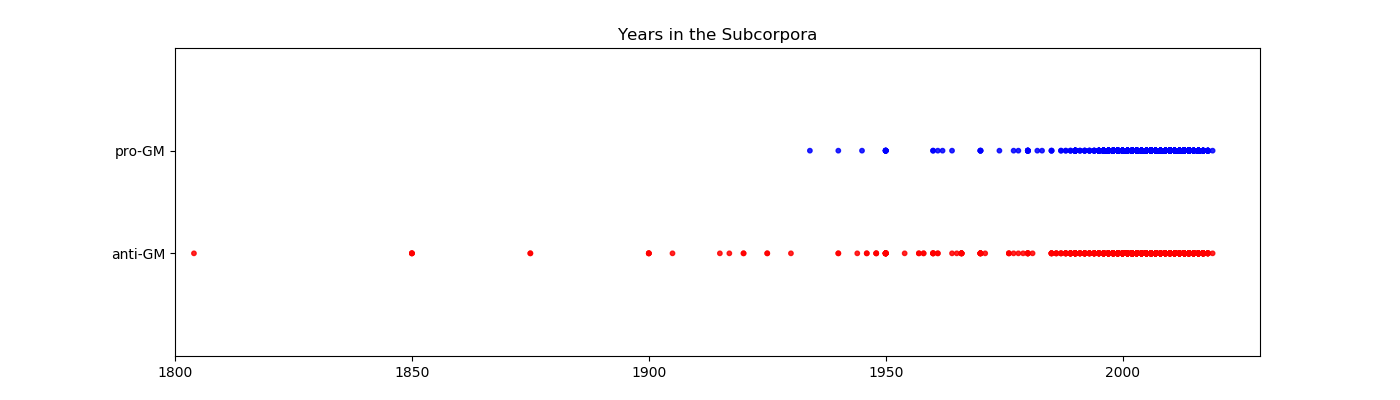
\includegraphics[width=16cm]{Figures/years.png}
\end{figure}

\section{Socio-Economic Context}

\textbf{Code: Concordances of \textit{income}}
\begin{lstlisting}
income_concord = []
income_concord_pro = []
getConcord("income", income_concord, income_concord_pro)
print('ANTI-GM Corpus' + "\n--------------" + "\n")                     
print("Total unique lines: " + str(len(income_concord)) + "\n")
print('Random sample:' + "\n") 
from random import sample
chosen_income = sample(income_concord, 10)
for i in chosen_income:
    print(i)
print('\nPRO-GM Corpus' + "\n--------------" + "\n")            
print("Total unique lines: " + str(len(income_concord_pro)) + "\n")
print('Random sample:' + "\n") 
from random import sample
chosen_income = sample(income_concord, 10)
for i in chosen_income:
    print(i)
\end{lstlisting}

\textbf{Output: Years in the Corpus}

\begin{footnotesize}

ANTI-GM Corpus\newline
--------------

Total unique lines: 58

Random sample:

y negative impact spread income farmer congress consideri\newline
ity rather lack adequate income access food country nativ\newline
hn resulted monsanto net income increasing million net in\newline
vailability access trade income generation purchasing foo\newline
 setting level necessary income also sought ensure farmer\newline
 rape sector canada lost income organic gm free producer \newline
 number household report income source outside community \newline
t climate change adapted income earning activity etc way \newline
ommodity price push farm income percent year billion lowe\newline
 bushel acre would meant income c end plant barley earned

PRO-GM Corpus\newline
--------------

Total unique lines: 237

Random sample:

ure livelihood outcome r income e increased wellr reduced\newline
overall effect crop farm income negative feedback farmer \newline
ity rather lack adequate income access food country nativ\newline
ience ht crop translated income benefit positive aspect i\newline
 agrochemical use farmer income look indirect impact deve\newline
rent indigenousgenerated income earning activity member a\newline
odity price pushing farm income expected lowest level six\newline
hn resulted monsanto net income increasing million net in\newline
vailability access trade income generation purchasing foo\newline
d reduce potential gross income sale fewer larger farm re

\end{footnotesize}

\textbf{Code: Collocates of \textit{corporate}}
\begin{lstlisting}
corporate_concord = []
corporate_concord_pro = []
corp_anti = []
corp_pro = []
getConcordWildcard(anti_file, 'corporate', corporate_concord) 
getConcordWildcard(pro_file, 'corporate', corporate_concord_pro) 
def getCorp(lst1, lst2):
    for i in lst1:
        if len(i) > 1:
            j=i.split()
            if("corporate" in j):
                ind = j.index("corporate")
                s = j[ind+1]
                s = re.sub(r'[^\w\s]','',s)
                lst2.append(s)
    d1a = dict()
    for i in lst2:
      d1a[i] = d1a.get(i, 0) + 1
    sorted_d1a = sorted(d1a.items(), key=operator.itemgetter(1), reverse=True)
    out = []
    for key, value in sorted_d1a:
        if value>1:
            out.append([key, value])
    print(tabulate(out, headers=['Collocate', 'Freq.']))
print('ANTI-GM Corpus:' + "\n")                     
print("Total unique lines: " + str(len(corporate_concord)) + "\n")
getCorp(corporate_concord, corp_anti)      
print('\nPRO-GM Corpus:' + "\n")            
print("Total unique lines: " + str(len(corporate_concord_pro)) + "\n")
getCorp(corporate_concord_pro, corp_pro) 
\end{lstlisting}

\textbf{Output: Collocates of \textit{corporate}}

\begin{footnotesize}
ANTI-GM Corpus:

Total unique lines: 87
\end{footnotesize}

\begin{table}[H]
\begin{footnotesize}
\begin{tabular}{ll}
\textbf{Collocate} & \textbf{Freq.} \\
sector             & 10             \\
control            & 8              \\
power              & 4              \\
seed               & 4              \\
agriculture        & 3              \\
sectors            & 2              \\
greed              & 2              \\
subsidies          & 2              \\
takeover           & 2              \\
consolidation      & 2             
\end{tabular}
\end{footnotesize}
\end{table}
\begin{footnotesize}
Pro-GM Corpus:

Total unique lines: 23
\end{footnotesize}

\begin{table}[H]
\begin{footnotesize}
\begin{tabular}{ll}
\textbf{Collocate} & \textbf{Freq.} \\
watch      & 2             
\end{tabular}
\end{footnotesize}
\end{table}


\textbf{Code: Income Split}

\begin{lstlisting}
gdp_file = "C:...\gdp.csv"
import pandas
colnames1 = ["rank","country","gdp"]
data_gdp = pandas.read_csv(gdp_file, names=colnames1)
rank_gdp = data_gdp["rank"].tolist()
countries_gdp = data_gdp["country"].tolist()
gdp = data_gdp["gdp"].tolist()
countries_gdp = [w.replace('\xa0', '') for w in countries_gdp]
ranks = dict(zip(countries_gdp, rank_gdp))
gdps = dict(zip(countries_gdp, gdp))
quart = int(0.25*len(countries_gdp))
quartile_top = countries_gdp[0:quart]
quartile_bottom = countries_gdp[2*quart:4*quart]
def sumRanks(dic, master):
    keysC = []
    valuesC = []
    countr = []
    sorted_dic = sorted(dic.items(), key=operator.itemgetter(1), reverse=True)
    for key, value in sorted_dic:
        keysC.append(countries.get(key)[0])
        valuesC.append(value)
        if countries.get(key)[0] not in countries_gdp:
            print(countries.get(key)[0])
    tot_dic = 0
    for c in master:
        tot_dic=tot_dic+int(ranks.get(c))
    print("avg rank: " + str(int(tot_dic/len(master))))
    tot_gdp = 0
    for c in master:
        #print(c)
        tot_gdp=tot_gdp+int(gdps.get(c))
    print("avg gdp " + str(round(tot_gdp/len(master),2)))
    count_top = 0
    count_bottom = 0
    for c in master:
        if c in quartile_top:
            count_top = count_top+1
        if c in quartile_bottom:
            count_bottom = count_bottom+1 
    print("% in top quartile: " + str(100*round(count_top/len(master),2)))
    print("% in bottom quartile: " + str(100*round(count_bottom/len(master),2)))
    #print(len(keysC))
print('ANTI-GM Corpus' + "\n")  
sumRanks(freq_anti, master_anti)
print("\n"+'PRO-GM Corpus' + "\n")  
sumRanks(freq_pro, master_pro)

\end{lstlisting}


\textbf{Output: Income Split}

\begin{footnotesize}
ANTI-GM Corpus

avg rank: 90\newline
avg GDP: 20765.94\newline
\% in top quartile: 32.0\newline
\% in bottom quartile: 38.0

PRO-GM Corpus

avg rank: 81\newline
avg GDP: 22370.72\newline
\% in top quartile: 35.0\newline
\% in bottom quartile: 32.0
\end{footnotesize}